\chapter{Analisi non distributive}
Le analisi distributive sono analisi statiche che si basano su ciò che viene 
calcolato, entrando quindi nel merito del valore che viene attribuito alle variabili 
cercando proprietà su tali valori.
\section{Propagazione delle costanti}
La propagazione delle costanti è un'analisi che ha come obiettivo quello di determinare 
se una variabile ha sempre lo stesso valore in un certo punto di programma.

Dato un punto di programma $p$, determina se una variabile nel punto di programma $p$ è sempre 
un valore costante. Tale analisi collegata alla \textbf{valutazione parziale}, che in un certo senso, 
che è collegata al concetto di \textbf{specializzazione}, discusso nell'ambito dei linguaggi 
di programmazione.

Cerchiamo quindi di capire se in un certo punto di programma una variabile ha sempre
lo stesso valore e in questo caso è possibile utilizzare tale valore per valutare parzialmente 
il programma preso in considerazione, vedendo quindi se alcuni dei calcoli possono essere
elaborati in funzione di un valore costante che il programma in quel punto di programma assume.

In un caso pratico, se in un certo
punto di programma una variabile che è utilizzata come condizione di un \textit{branching},
assume sempre lo stesso valore, talvolta è possibile eliminare il \textit{branching} e
eseguire solo una delle due parti del \textit{branching}.

\begin{algorithm}[H]
    $x \gets 1$\;
    \dots\;
    \If{$x > 0$}{
        $e$\;
    }
    \Else{
        $e'$\;
    }
\end{algorithm}
\begin{algorithm}[H]
    $x \gets 1$\;
    \dots\;
    $e$\;
\end{algorithm}

In questo senso l'informazione può essere utilizzata in vari ambiti permettendoci inoltre 
di capire quali valori possono assumere le variabili in un certo punto di programma.
Come \textit{side effect} di tale analisi, possiamo inoltre capire se un punto di 
programma è raggiungibile o meno.
\subsubsection{Esempio}
Supponiamo di avere il seguente programma:

\begin{algorithm}[H]
    $a:=1; b:=2; c:=3; d:=3; e:=0$\;
    \While{$B$}
    {
        $b := 2 \cdot a; d:=d+1; e:=e-a$\;
        $c :=e + d; a:= b - a$\;
    }
\end{algorithm}
Dove $B$ indica che la condizione sul ciclo non è nota staticamente.
Verifichiamo lo stato delle variabili dopo ogni punto di programma:
\begin{figure}[H]
    \centering
    \begin{tabular}{c|ccccc}
        & \texttt{a} &\texttt{b} & \texttt{c} & \texttt{d} & \texttt{e} \\
        \hline
        \textbf{1} & $1$ & $2$ & $3$ & $3$ & $0$ \\
        \textbf{2} & $1$ & $2$ & $3$ & \redtext{$3$} & \redtext{$0$} \\
        \textbf{3} & $1$ & $2$ & $3$ & $4$ & $-1$ \\
        \textbf{4} & $1$ & $2$ & $3$ & \redtext{$4$} & \redtext{$-1$} \\
        \hline
        \textbf{1} & $1$ & $2$ & $3$ & $3$ & $0$ \\
        \textbf{2} & $1$ & $3$ & $3$ & $?$ & $?$ \\
        \textbf{3} & $1$ & $3$ & $2$ & $?$ & $?$ \\
        \textbf{4} & $2$ & $3$ & $?$ & $?$ & $?$ \\
    \end{tabular}
\end{figure}
Dopo la prima iterazione, al punto di programma $2$, viene collezionato 
ciò che viene fatto al punto di programma $4$, visto che dal punto $4$ si ritorna al punto $2$
data la presenza del ciclo.

Collezionando valori vediamo che variano sono i valori di $d$ e $e$, quindi 
non possiamo dire nulla sui loro valori. Calcolando il valore di $d$, viene 
eseguita una somma con un valore non conosciuto, quindi $?$ non può essere
a sua volta conosciuto.

Concludiamo quindi che non possiamo dire nulla sul valore di $c$, $d$ e $e$, 
mentre possiamo dire che $a$ e $b$ sono sempre uguali a $1$ e $2$ rispettivamente.
A differenza dell'analisi astratta, nel caso concreto il valore di $c$ sarebbe 
sempre $3$, di fatto costante.
\subsection{Costruzione dell'analisi}
Il primo passo per costruire l'analisi è quello di definire il dominio delle 
informazioni astratte, ovvero delle proprietà che vogliamo osservare con precisione.

Nel dominio concreto $\mathcal{C}= \wp(\mathbb{Z})$, lavoriamo su valori interi, 
insiemi di interi. Tra questi insiemi di interi, l'obiettivo è osservare con 
precisione i singoletti, quindi:
\[
    \mathcal{A} = \{n \mid n \in \mathbb{Z}\} \cup \{\bot, \top\} = \mathbb{Z}^\top
\]

Dal momento in cui una variabile colleziona più di un valore possibile,
l'informazione non è più precisa, quindi non è più possibile dire nulla 
sul fatto che possa essere costante o meno.

L'inserzione di Galois tra i due domini $\mathcal{C}$ e $\mathcal{A}$ è 
data dalle funzioni: 
\[
    \alpha(x) = 
    \begin{cases}
        \top & \text{se } x = \varnothing \\
        n & \text{se } S = \{n\} \quad n\in \mathbb{Z} \\
        \top & \text{altrimenti}
    \end{cases}
\]
\[
    \gamma(a) = 
    \begin{cases}
        \varnothing & \text{se } a = \top \\
        \{n\} & \text{se } a = n \quad n\in \mathbb{Z} \\
        \mathbb{Z} & \text{altrimenti}
    \end{cases}
\]
dove $x \in \wp(\mathbb{Z})$ e $a \in \mathcal{A}$ e
con $\alpha$ che è la funzione di astrazione e $\gamma$ che è la funzione di concretizzazione, 
entrambe funzioni monotone; si può dimostrare che formano una \textit{inserzione di Galois}.
\begin{figure}[H]
    \centering
    \begin{tikzpicture}
        \node (top) at (0, 2) {$\top$};
        \node (f1) at (6, 0) {$\dots$};
        \node (z) at (4, 0) {$2$};
        \node (a) at (2, 0) {$1$};
        \node (c) at (0, 0) {$0$};
        \node (e) at (-2, 0) {$-1$};
        \node (f2) at (-4, 0) {$-2$};
        \node (f3) at (-6, 0) {$\dots$};
        \node (bot) at (0, -2) {$\bot$};

        % Linee verso \top
        \draw (z.north) -- (top.south);
        \draw (a.north) -- (top.south);
        \draw (c.north) -- (top.south);
        \draw (e.north) -- (top.south);
        \draw (f2.north) -- (top.south);

        % Linee verso \bot
        \draw (z.south) -- (bot.north);
        \draw (a.south) -- (bot.north);
        \draw (c.south) -- (bot.north);
        \draw (e.south) -- (bot.north);
        \draw (f2.south) -- (bot.north);
    \end{tikzpicture}
    \caption{Rappresentazione grafica del dominio delle costanti $\mathbb{Z}^\top$}
\end{figure}
Dati $x,y \in \mathbb{Z}^\top$ se e solo se $x \sqsubseteq y$ oppure $y=\top$ o $x=\bot$.
È chiaro che si tratti di un \textbf{astrazione dei valori}, ma la semantica opera su stati, 
quindi l'obiettivo è di estendere il dominio delle costanti a quello degli stati, su cui 
calcoleremo la semantica astratta.

Se lo stato è una funzione da variabili a valori, $\sigma : \texttt{Var} \to \mathbb{Z}$; 
nel caso collecting, $S : \texttt{Var} \to \wp(\mathbb{Z})$. Lo stato astratto sarà quindi
una funzione $\mathbb{D}$ all'astrazione di parti di $\mathbb{Z}$, ovvero 
\[
    \mathbb{D} : \texttt{Var} \to \mathbb{Z}^\top 
\]
Definiamo quindi il dominio degli stati astratti nelle costanti come 
\[
    \mathbb{D} = (\texttt{Var} \to \mathbb{Z}^\top) \cup \{\bot\}
\] 
Dove $\bot$ è un elemento che rappresenta i punti non raggiungibili, che sarà ovviamente minore 
di ogni memoria del dominio.
Definiamo $\mathbb{D}_\bot \stackrel{\tiny def}{=} \forall x . x \mapsto \bot$, ovvero la memoria 
che associa ad ogni variabile il valore $\bot$, dove quindi nessuna variabile è stata inizializzata.

Questo è quindi il dominio dove definiamo la semantica astratta, tale dominio è \textit{pointwise},
ovvero il confronto tra due stati astratti è dato dal confronto tra i valori delle variabili.
\[
    \mathcal{D}_1 \sqsubseteq \mathcal{D}_2 \iff \forall x \in \texttt{Var} . 
    \mathcal{D}_1(x) \sqsubseteq_{const} \mathcal{D}_2(x)
\]
Confrontiamo due funzioni, confrontando l'immagine delle due funzioni per ogni singola 
variabile. Tale ordinamento permette di definire il \textit{least upper bound} come:
\[
    \texttt{Lub} : \bigsqcup_i \mathcal{D}_i(x) =
    \begin{cases}
        z & \text{se } \forall i . \mathcal{D}_i(x) = z \qquad z \in \mathbb{Z} \\
        \top & \text{altrimenti}
    \end{cases}
\]
Con questo ordinamento, $\mathbb{D}$ è un reticolo completo, ed è quindi il dominio
astratto per le costanti.

A questo punto possiamo iniziare a capire cosa vogliamo calcolare nella nostra analisi,
esattamente come abbiamo fatto nell'analisi di \textit{data flow}, vogliamo fornire una 
semantica astratta dei programmi nel dominio astratto $\mathbb{D}$, quindi una funzione
\[
\forall \mathcal{D} \in \mathbb{D} . \llbracket \cdot \rrbracket^\sharp \mathcal{D}
\]
Che dice se ogni variabile è costante o meno. L'obiettivo è avere questa informazione 
per ogni punto di programma, quindi cerchiamo la soluzione \texttt{MOP}, ovvero la
soluzione \textit{merge over all paths}, definendo quindi:
\[
    \texttt{MOP} : \mathcal{D}^\star [v] = \bigsqcup 
    \{ \llbracket \pi \rrbracket^\sharp \mathcal{D}_\bot \mid \pi:\text{start} \to v \}
\]
Ovvero il \textit{least upper bound}  (\textit{poiché la collecting semantics è di tipo possible}) 
delle semantiche di tutti i cammini a partire dall'informazione iniziale $\mathcal{D}_\bot$
dei cammini 
che vanno dal nodo di inizio al nodo $v$. È chiaro che se guardiamo tale analisi dal punto di vista delle 
analisi di data flow, l'analisi è forward, ed è di tipo possibile perché colleziona valori.

Dobbiamo quindi definire la semantica approssimata sugli stati astratti
$\llbracket \cdot \rrbracket^\sharp$, considerando 
il fatto che i nostri archi sono della forma $(u, \texttt{lab}, v)$, considerando che la 
semantica è fornita dall'etichetta dell'arco, a partire dalla memoria $\mathcal{D}$ astratta 
che raggiunge il nodo $u$, quindi $\llbracket \texttt{lab} \rrbracket^\sharp : \mathcal{D}$. 
\subsection{Semantica delle espressioni} \label{sec:semantica-espressioni}
La prima cosa che conviene fare è andare a trasferire il calcolo delle operazioni concrete 
nel dominio astratto, quindi definiamo la funzione di trasferimento astratta.
Per farlo definiamo l'operazione generica $\square$ su interi e la sua versione astratta
$\square^\sharp$ su $\mathbb{Z}^\top$.

\[
  a,b \in \mathbb{Z}^\top \quad . \quad a \square^\sharp b =
  \begin{cases}
    \top & \text{se } a = \top \lor b = \top \\
    a\, \square\, b & \text{altrimenti}
  \end{cases}
\]
Si tratta esattamente della \textbf{best correct approximation} dell'operazione $\square$, 
perché prendere nel concreto l'operazione $\square$ equivale a farla per tutti gli elementi 
dei due insiemi, equivalente quindi al singoletto, per poi tornare nel dominio astratto 
e osservare il signoletto.

Una volta definita l'operazione astratta possiamo definire la semantica delle espressioni, 
$\llbracket e \rrbracket ^\sharp \mathcal{D}$ ovvero la semantica approssimata a partire da una memoria $\llbracket e \rrbracket^\sharp :
\mathcal{D} \to \mathbb{Z}^\top$. Nella analisi di data flow non è stata definita poiché 
non è mai interessato il valore restituito dalla valutazione di un'espressione, ma solo
la struttura sintattica del programma. Nelle analisi di tipo distributive, dove il valore delle 
variabili è parte dell'analisi, è necessario definire la semantica delle espressioni perché 
la valutazione restituisce un valore appartenente al dominio astratto, quindi è necessario
per l'analisi.

Ragioniamo quindi induttivamente sulla struttura della semantica 
astratta delle espressioni, definendo la semantica:
\begin{itemize}
  \item $c \in \mathbb{Z} . \llbracket c \rrbracket^\sharp \mathcal{D} = c$
  \item $x \in \texttt{Var} . \llbracket x \rrbracket^\sharp \mathcal{D} =
  \mathcal{D}(x) \in \mathbb{Z}^\top$
  \item $\llbracket \square e \rrbracket^\sharp \mathcal{D} =
  \square^\sharp \llbracket e \rrbracket^\sharp \mathcal{D}$
  \item $\llbracket e_1 \square e_2 \rrbracket^\sharp \mathcal{D} = 
  \llbracket e_1 \rrbracket^\sharp \mathcal{D} \square^\sharp \llbracket e_2 \rrbracket^\sharp \mathcal{D}$
\end{itemize}
\subsubsection{Esempio di valutazione di un'espressione astratta}
Consideriamo la seguente espressione:
\[
  \mathcal{D} = [x \mapsto 2, y \mapsto \top] 
\]
\[ 
    \llbracket x + 7 \rrbracket^\sharp \mathcal{D} =
    \llbracket x \rrbracket^\sharp \mathcal{D} +^\sharp 
    \llbracket 7 \rrbracket^\sharp \mathcal{D} =
    \mathcal{D}(x) +^\sharp 7 = 2 +^\sharp 7 = 9
\]
Consideriamo ora la seguente espressione:
\[
  \llbracket x + y \rrbracket^\sharp \mathcal{D} =
    \llbracket x \rrbracket^\sharp \mathcal{D} +^\sharp
    \llbracket y \rrbracket^\sharp \mathcal{D} =
    \mathcal{D}(x) +^\sharp \mathcal{D}(y) = 2 +^\sharp \top = \top
\]
\subsection{Semantica dei comandi}
La semantica dei comandi ovviamente si baserà sulla semantica delle espressioni 
nel caso delle guardie e dell'assegnamento. Ragioniamo quindi induttivamente sulla
struttura dei comandi, definendo la semantica astratta dei comandi:
\begin{itemize}
    \item $\llbracket \texttt{;} \rrbracket^\sharp \mathcal{D} = \mathcal{D}$
    \item Se il ramo non è percorribile allora utilizzeremo il valore $\bot$, 
    se invece lo è lasceremo la memoria invariata.
    Quindi non sarà percorribile quando nessun valore che rende vero il test è 
    presente tra i possibili valori che abbiamo calcolato per $e$. Poiché per $e$  
    è possibile calcolare o è un valore costante o è $\top$, allora non è percorribile
    quando la valutazione di $e$ è esattamente $0$.
    \[
        \llbracket \texttt{NonZero(e)} \rrbracket^\sharp \mathcal{D} = 
        \begin{cases}
            \bot & \text{se } \llbracket e \rrbracket^\sharp \mathcal{D} = 0 \\
            \mathcal{D} & \text{altrimenti } (\exists n \not = 0 . 
            \llbracket e \rrbracket^\sharp \mathcal{D} = n \lor
            \llbracket e \rrbracket^\sharp \mathcal{D} = \top)
        \end{cases}  
    \]
    \item Abbiamo un caso analogo per il ramo \texttt{Zero}, sicuramente il rmo non sarà percorribile 
    quando $0$ non è contenuto all'interno di $e$.
    
    \[
      \llbracket \texttt{Zero(e)} \rrbracket^\sharp \mathcal{D} =
        \begin{cases}
            \bot & \text{se } \llbracket e \rrbracket^\sharp \mathcal{D} \not\sqsubseteq 0 \\
            \mathcal{D} & \text{altrimenti } (\llbracket e \rrbracket^\sharp \mathcal{D}
            = 0 \lor \llbracket e \rrbracket^\sharp \mathcal{D} = \top)
        \end{cases}  
    \]
    \item In caso di assegnamento andiamo a calcolare il valore astratto associato all'espressione 
    e aggiorniamo la memoria astratta con tale valore.
    \[
      \mathcal{D}[x \mapsto \llbracket e \rrbracket^\sharp \mathcal{D}]
    \]
    \item Con l'input sappiamo il valore che $x$ assume solamente a tempo di esecuzione, nonostante 
    si sappia il fatto che sicuramente assumerà un unico valore.
    \[
      \llbracket \texttt{input x} \rrbracket^\sharp \mathcal{D} = \mathcal{D}[x \mapsto \top]  
    \]
\end{itemize}
Essendo una semantica forward, dato un cammino $\pi = k_0 \dots k_n$, sappiamo che
$\llbracket \pi \rrbracket^\sharp = \llbracket k_n \rrbracket^\sharp \circ \dots \circ
\llbracket k_0 \rrbracket^\sharp \mathcal{D}_\bot$, la semantica approssimata del cammino, 
sarà la composizione delle semantica approssimata dei singoli comandi a partire da una 
memoria iniziale $\mathcal{D}_\bot$, dove la semantica di un arco è esattamente 
la semantica approssimata della sua etichetta $\llbracket \texttt{lab}_n \rrbracket^\sharp$.

Si può dimostrare che la semantica astratta $\llbracket \cdot \rrbracket^\sharp$ non 
è distributiva, quindi calcolando la soluzione \texttt{MFP} questa non sarà uguale 
alla soluzione \texttt{MOP}, ma la contiene strettamente.
\[
  \texttt{MFP} \sqsupseteq \texttt{MOP}  
\]
In ogni caso, la soluzione \texttt{MFP} è l'unica che riusciamo a costruire e l'analisi 
costruisce tale soluzione. 
Per farlo trova la soluzione del sistema di disequazioni, costruito esattamente come nel 
caso della analisi di data flow.
\begin{itemize}
    \item Sul nodo di partenza la memoria astratta è vuota, quindi
    \[
        \mathcal{D}[\texttt{entry}] \sqsupseteq \mathcal{D}_\bot 
    \]
    \item Per i nodi successivi, essendo una semantica forward, $\mathcal{D}[v]$ contiene 
    la semantica dell'etichetta a partire dalla memoria astratta a 
    partire dal nodo sorgente.
    \[
        \mathcal{D}[v] \sqsupseteq \llbracket \texttt{lab} \rrbracket^\sharp \mathcal{D}[u]
    \]
\end{itemize}
In ogni caso la semantica $\llbracket \cdot \rrbracket^\sharp$ è monotona e il 
dominio è \texttt{ACC}, data l'altezza finita, e quindi la soluzione \texttt{MFP} 
esiste ed è calcolabile.
\subsubsection{Esempio di non distributività}
Consideriamo le seguenti memorie astratte:
\[
    \mathcal{D}_1 = \{ x \mapsto 2, y \mapsto 3 \} \qquad
    \mathcal{D}_2 = \{ x \mapsto 3, y \mapsto 2 \}
\]
e vediamo cosa succede nel calcolo:
\[
    \llbracket x \gets x + y \rrbracket^\sharp \mathcal{D}_1 
    \,\bigsqcup\, 
    \llbracket x \gets x + y \rrbracket^\sharp \mathcal{D}_2
\]
A sinistra abbiamo:
Quindi 
\[
    \mathcal{D}_1 [x \mapsto 5] \qquad \mathcal{D}_1 = \{ x \mapsto 5, y \mapsto 3 \}
\]
A destra abbiamo:
\[
    \mathcal{D}_2 [x \mapsto 5] \qquad \mathcal{D}_2 = \{ x \mapsto 5, y \mapsto 2 \}
\]
Se facciamo il least upper bound otteniamo 
\[
    \mathcal{D}_1 \,\bigsqcup\, \mathcal{D}_2 = 
    \{ x \mapsto 5, y \mapsto 3 \} \,\bigsqcup\, \{ x \mapsto 5, y \mapsto 2 \} = 
    \{ x \mapsto 5, y \mapsto \top \}
\]
Calcolando la semantica combinando le due memorie astratte otteniamo:
\[
    \llbracket x \gets x + y \rrbracket^\sharp (\mathcal{D}_1 \,\bigsqcup\, \mathcal{D}_2) = 
    \llbracket x \gets x + y \rrbracket^\sharp \{ x \mapsto \top, y \mapsto \top \} =
    \{ x \mapsto \top, y \mapsto \top \}
\]
quindi:
\begin{tcolorbox}[title = Non distributività della semantica]
    Non possiamo calcolare precisamente la combinazione della semantica dei cammini
    come semantica delle combinazioni locali delle memorie raggiunte.
    \[
        \llbracket x \gets x + y \rrbracket^\sharp \mathcal{D}_1
        \,\bigsqcup\,
        \llbracket x \gets x + y \rrbracket^\sharp \mathcal{D}_2
        \,\not \sqsubseteq\,
        \llbracket x \gets x + y \rrbracket^\sharp (\mathcal{D}_1 \,\bigsqcup\, \mathcal{D}_2)
    \]
\end{tcolorbox}
\subsubsection{Esempio di analisi della propagazione delle costanti}

\begin{minipage}{0.5\textwidth}
    Riportiamo il programma programma precedentemente analizzato.

    \begin{algorithm}[H]
        $a:=1; b:=2; c:=3; d:=3; e:=0$\;
        \While{$B$}
        {
            $b := 2 \cdot a; d:=d+1; e:=e-a$\;
            $c :=e + d; a:= b - a$\;
        }
    \end{algorithm}
\end{minipage}
\begin{minipage}{0.5\textwidth}
    \begin{figure}[H]
        \centering
        \begin{tikzpicture}[node distance={22mm}, minimum width = 1cm, main/.style = {draw, circle}] 
            \node[main] (1) {1};
            \node[main] (2) [below =of 1] {2};
            \node[main] (3) [below right =of 2] {3};
            \node[main] (4) [below =of 3] {4};
            \node[main] (5) [below left=of 2] {5};

            \draw[->] (1) -- (2) node[midway, right] {$\texttt{lab}_1$};
            \draw[->] (2) -- (5) node[midway, left] {$\texttt{Zero}(B)$};
            \draw[->] (2) -- (3) node[midway, right] {$\texttt{NonZero}(B)$};
            \draw[->] (3) -- (4) node[midway, right] {$\texttt{lab}_3$};
            \draw[->] (4) -- (2) node[midway, left] {$\texttt{lab}_4$};
        
        \end{tikzpicture}
    \end{figure}
\end{minipage}
Dobbiamo costruire il sistema di disequazioni:
\begin{itemize}
    \item $ \mathcal{D}(1) \sqsupseteq \mathcal{D}_\bot$
    \item $ \mathcal{D}(2) \sqsupseteq [\texttt{a} \mapsto 1, \texttt{b} 
    \mapsto 2, \texttt{c} \mapsto 3, \texttt{d} \mapsto 3, \texttt{e} \mapsto 0] 
    \sqcup \mathcal{D}(4)[a \mapsto \mathcal{D}(4)(a) -^{\sharp} \mathcal{D}(4)(b), 
    c \mapsto \mathcal{D}(4)(e) +^{\sharp} \mathcal{D}(4)(d)]$
    \item $ \mathcal{D}(3) \sqsupseteq \mathcal{D}(2)$
    \item $ \mathcal{D}(4) \sqsupseteq \mathcal{D}(3)[b \mapsto 2 \cdot^{\sharp} 
    \mathcal{D}(3)(a), d \mapsto \mathcal{D}(3)(d) +^{\sharp} 1, 
    e \mapsto \mathcal{D}(3)(e) -^{\sharp} \mathcal{D}(3)(a)]$
    \item $ \mathcal{D}(5) \sqsupseteq \mathcal{D}(2)$
\end{itemize} 
Nel least upper bound accorpiamo i vari archi che arrivano allo stesso punto, quindi 
la minima soluzione del sistema di disequazioni diventa uguale alla soluzione del
sistema di equazioni.
\begin{itemize}
    \item $ \mathcal{D}(1) = \mathcal{D}_\bot$
    \item $ \mathcal{D}(2) = [\texttt{a} \mapsto 1, \texttt{b} 
    \mapsto 2, \texttt{c} \mapsto 3, \texttt{d} \mapsto 3, \texttt{e} \mapsto 0] 
    \sqcup \mathcal{D}(4)[a \mapsto \mathcal{D}(4)(b) -^{\sharp} \mathcal{D}(4)(a), 
    c \mapsto \mathcal{D}(4)(e) +^{\sharp} \mathcal{D}(4)(d)]$
    \item $ \mathcal{D}(3) = \mathcal{D}(2)$
    \item $ \mathcal{D}(4) = \mathcal{D}(3)[b \mapsto 2 \cdot^{\sharp} 
    \mathcal{D}(3)(a), d \mapsto \mathcal{D}(3)(d) +^{\sharp} 1, 
    e \mapsto \mathcal{D}(3)(e) -^{\sharp} \mathcal{D}(3)(a)]$
    \item $ \mathcal{D}(5) = \mathcal{D}(2)$
\end{itemize} 
Procediamo con la soluzione del sistema di equazioni:
\begin{table}[H]
    \centering
    \begin{subtable}{\linewidth}
        \centering
        \begin{tabular}{|c|c|c|c|}
            \hline
            & $0$ 
            & $1$ 
            & $2$ \\ \hline
            $\mathcal{D}(1)$ 
            & $\mathcal{D}_\bot$ 
            & $\mathcal{D}_\bot$ 
            & $\mathcal{D}_\bot$ \\
            \hline
            $\mathcal{D}(2)$ 
            & $\varnothing$ 
            & $\texttt{a} \mapsto 1, \texttt{b} \mapsto 2, \texttt{c} \mapsto 3, \texttt{d} \mapsto 3, \texttt{e} \mapsto 0$ 
            & $\texttt{a} \mapsto 1, \texttt{b} \mapsto 2, \texttt{c} \mapsto 3, \texttt{d} \mapsto \top, \texttt{e} \mapsto \top$ \\
            \hline
            $\mathcal{D}(3)$ 
            & $\varnothing$ 
            & $\texttt{a} \mapsto 1, \texttt{b} \mapsto 2, \texttt{c} \mapsto 3, \texttt{d} \mapsto 3, \texttt{e} \mapsto 0$ 
            & $\texttt{a} \mapsto 1, \texttt{b} \mapsto 2, \texttt{c} \mapsto 3, \texttt{d} \mapsto \top, \texttt{e} \mapsto \top$ \\
            \hline
            $\mathcal{D}(4)$ 
            & $\varnothing$ 
            & $\texttt{a} \mapsto 1, \texttt{b} \mapsto 2, \texttt{c} \mapsto 3, \texttt{d} \mapsto 4, \texttt{e} \mapsto -1$ 
            & $\texttt{a} \mapsto 1, \texttt{b} \mapsto 2, \texttt{c} \mapsto 3, \texttt{d} \mapsto \top, \texttt{e} \mapsto \top$ \\
            \hline
            $\mathcal{D}(5)$ 
            & $\varnothing$ 
            & $\texttt{a} \mapsto 1, \texttt{b} \mapsto 2, \texttt{c} \mapsto 3, \texttt{d} \mapsto 3, \texttt{e} \mapsto 0$ 
            & $\texttt{a} \mapsto 1, \texttt{b} \mapsto 2, \texttt{c} \mapsto 3, \texttt{d} \mapsto \top, \texttt{e} \mapsto \top$ \\
            \hline
        \end{tabular}
    \end{subtable}
    
    \vspace{1cm}
    
    \begin{subtable}{\linewidth}
        \centering
        \begin{tabular}{|c|c|}
            \hline
            & $3$ \\
            \hline
            $\mathcal{D}(1)$
            & $\mathcal{D}_\bot$ \\
            \hline
            $\mathcal{D}(2)$ 
            & $\texttt{a} \mapsto 1, \texttt{b} \mapsto 2, \texttt{c} \mapsto \top, \texttt{d} \mapsto \top, \texttt{e} \mapsto \top$ \\
            \hline
            $\mathcal{D}(3)$ 
            & $\texttt{a} \mapsto 1, \texttt{b} \mapsto 2, \texttt{c} \mapsto \top, \texttt{d} \mapsto \top, \texttt{e} \mapsto \top$ \\
            \hline
            $\mathcal{D}(4)$ 
            & $\texttt{a} \mapsto 1, \texttt{b} \mapsto 2, \texttt{c} \mapsto \top, \texttt{d} \mapsto \top, \texttt{e} \mapsto \top$ \\
            \hline
            $\mathcal{D}(5)$ 
            & $\texttt{a} \mapsto 1, \texttt{b} \mapsto 2, \texttt{c} \mapsto \top, \texttt{d} \mapsto \top, \texttt{e} \mapsto \top$ \\
            \hline
        \end{tabular}
    \end{subtable}
\end{table}
Raggiungiamo il punto fisso alla terza iterazione.
Di fatto in funzione dell'analisi osserviamo che l'informazione persa è quella 
relativa alla variabile $c$ rispetto al calcolo concreto. Infatti nel calcolo 
concreto il suo valore è costante, ma nel calcolo astratto dipende da variabili 
che nel calcolo astratto sono $\top$.
\subsection{Migliorie dell'analisi}
Possiamo pensare di migliorare l'analisi sapendo che la presenza di guardie la cui 
informazione calcolata è rappresentabile all'interno della nostra osservazione; per capirlo 
osserviamo il seguente esempio:

\begin{algorithm}[H]
    \If{$x = 7$}{
        $e_1$\;
    }
\end{algorithm}
All'interno del ramo $e_1$ è possibile considerare
l'informazione relativa al fatto che il valore di $x$ è $7$.
Tale informazione è rappresentabile nel dominio delle costanti e utilizzarlo per il calcolo 
successivo.

Ovviamente il concetto riguarda le guardie la cui informazione è osservabile 
all'interno del ramo di esecuzione.
In questo caso rappresentiamo la semantica con tali migliorie nel seguente modo:

 \[
        \llbracket \texttt{NonZero(e)} \rrbracket^\sharp \mathcal{D} = 
        \begin{cases}
            \bot & \text{se } \llbracket e \rrbracket^\sharp \mathcal{D} = 0 \\
            \mathcal{D}_1 & \text{altrimenti } (\exists n \not = 0 . 
            \llbracket e \rrbracket^\sharp \mathcal{D} = n \lor
            \llbracket e \rrbracket^\sharp \mathcal{D} = \top)
        \end{cases}  
\]
Dove $\mathcal{D}_1 = \mathcal{D}[x \mapsto \mathcal{D}(x)
\sqcap \llbracket e \rrbracket^\sharp \mathcal{D}] = \llbracket e \rrbracket^\sharp \mathcal{D}$
Poiché si tratta di un'informazione di uguaglianza, quello che sappiamo è che nel raggio di 
azione della guardia, il valore di $x$ è esattamente il valore della semantica.
\section{Analisi degli intervalli}
In generale quando ci interessa qualche proprietà più sofisticate perdiamo 
le condizioni di finitezza del dominio e talvolta l'\texttt{ACC}. In particolare 
nell'analisi degli intervalli, dove il dominio è 
infinito e non abbiamo l'\texttt{ACC}, quindi abbiamo 
catene ascendenti \textbf{infinite}.

Nel dominio degli intervalli ogni elemento è rappresentato da un oggetto nella 
forma $[l, u] = \{n \in \mathbb{Z} \mid l \leq n \leq u\}$, dove $l$ è il 
limite inferiore e $u$ è il limite superiore.
Tra questi valori abbiamo anche intervalli dove $l = -\infty$ e $u = +\infty$.
\[
  [l, +\infty] = \{n \in \mathbb{Z} \mid l \leq n\}  
\]
\[
  [-\infty, u] = \{n \in \mathbb{Z} \mid n \leq u\}
\]
Prendendo in considerazione un qualsiasi elemento $[l, u]$ del dominio,
siamo in grado di trovare una quantità infinita di elementi che sono maggiori
di $[l, u]$. Il calcolo del punto fisso lavora collezionando 
i valori che le variabili possono assumere durante l'esecuzione del programma e 
lavorare in un dominio non \texttt{ACC} significa che tale catena può divergere 
perché possiamo continuare ad aggiungere elementi senza trovare il punto fisso.

Si tratta di un caso, nella sua semplicità, che contiene tutte le difficoltà 
dell'analisi statica. Vediamone ora la costruzione nel dettaglio.
\subsection{Costruzione dell'analisi}
L'analisi degli intervalli non ha come obiettivo osservare l'insieme 
concreto dei valori raggiungibili durante l'esecuzione, ma solamente il range 
di valori che una variabile può acquisire in un certo punto del programma.
I punti di programma che sono solitamente interessanti sono quelli all'interno di 
un ciclo, essendo questi i punti in cui ci può essere un'evoluzione
del valore. Gli intervalli approssimano riempiendo i buchi tra i valori, e 
per questo sono insiemi convessi. Un chiaro esempio di convessità è 
il seguente.

Supponiamo che $x$ sia una variabile intera e
che assume i seguenti valori durante l'esecuzione del programma:
\[
    x \mapsto \{1, 5, 20, 35\}
\]
Nella nostra analisi, è chiaro che nell'analisi assumerà 
il seguente valore:
\[
  x \mapsto [1, 35]  
\]
Prendendo in considerazione elementi che in realtà non sono presenti nel
dominio concreto, rendendo di fatto l'insieme convesso.

La prima cosa da fare è definire il dominio degli elementi che vogliamo 
osservare con precisione.
\[
  \mathbb{I}  = \{ [l, u] \mid l \in \mathbb{Z} \cup \{-\infty\}, 
  u \in \mathbb{Z} \cup \{+\infty\}, l \leq u \}
\]
Nel dominio concreto abbiamo l'insieme di valori su $\mathbb{Z}$ che 
le variabili possono assumere, ovvero $\wp(\mathbb{Z})$.
Il secondo passo è assicurarci che il dominio $\mathbb{I}$
sia effettivamente un 
dominio astratto, ovvero che esista un'inserzione di Galois
tra il dominio concreto e quello astratto.

L'inserzione di Galois tra i due domini $\mathcal{C}$ e $\mathcal{A}$ è 
data dalle funzioni: 
\[
    \alpha(x) = 
    [\texttt{min}_\infty (x), \texttt{max}_\infty (x)] \in \mathbb{I}
\]
Dove le due funzioni $\texttt{min}_\infty$ e $\texttt{max}_\infty$ sono definite 
nel seguente modo:
\[
    \texttt{min}_\infty (x) = 
    \begin{cases}
        n \in x & \text{se } \forall n \in x . m \leq n \\
        -\infty & \text{altrimenti}
    \end{cases}
\]
\[
    \texttt{max}_\infty (x) = 
    \begin{cases}
        n \in x & \text{se } \forall n \in x . m \geq n \\
        +\infty & \text{altrimenti}
    \end{cases}
\]
Mentre la funzione $\gamma$ è definita nel seguente modo:
\[
    \gamma([l, u]) = \{n \in \mathbb{Z} \mid l \leq_\infty n \leq_\infty u\}
\]
Dove il pedice $\infty$ indica che:
\[
  \forall m . \quad -\infty \leq_\infty \qquad m \leq_\infty +\infty  
\]
Quello che si può dimostrare è che $\alpha$ e $\gamma$ costituiscono 
un'inserzione di Galois tra i due domini.
\[
  \wp(\mathbb{Z}) \galoiS{\alpha}{\gamma} \mathbb{I}
\]
Dato un qualunque insieme, esiste la miglior approssimazione possibile, 
quindi esiste sempre il più piccolo intervallo che contiene l'insieme 
di partenza.
\subsection{Operazioni del reticolo}
\begin{itemize}
    \item Ordinamento
    \[ 
        [l_1, u_1] \sqsubseteq [l_2, u_2] \iff l_1 \geq l_2 \land u_1 \leq u_2
    \]
    \begin{figure}[H]
        \centering
        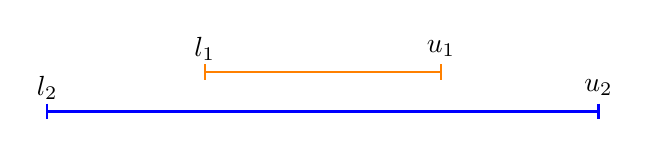
\begin{tikzpicture}
            %segmenti 
            \draw[thick, orange] (2, 0.5) -- (5, 0.5);
            \draw[thick, blue] (0, 0) -- (7, 0);
            \draw[thick, orange] (2, 0.6) -- (2, 0.4);
            \draw[thick, orange] (5, 0.6) -- (5, 0.4);
            \draw[thick, blue] (0, 0.1) -- (0, -0.1);
            \draw[thick, blue] (7, 0.1) -- (7, -0.1);
            %etichette
            \node at (2, 0.8) {$l_1$};
            \node at (5, 0.8) {$u_1$};
            \node at (0, 0.3) {$l_2$};
            \node at (7, 0.3) {$u_2$};
        \end{tikzpicture}
    \end{figure}
    \item Least upper bound: ovvero il più piccolo intervallo che contiene 
    entrambi gli intervalli.
    \[
        [l_1, u_1] \sqcup [l_2, u_2] = [\texttt{min}(l_1, l_2), \texttt{max}(u_1, u_2)]  
    \]
    \begin{figure}[H]
        \centering
        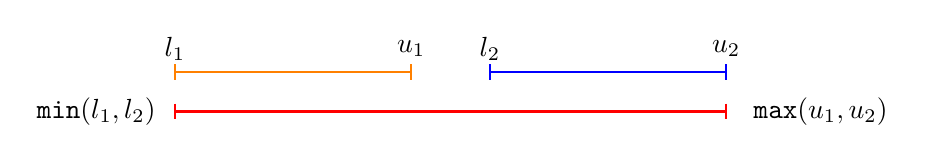
\begin{tikzpicture}
            %segmenti 
            \draw[thick, orange] (0, 0.5) -- (3, 0.5);
            \draw[thick, blue] (4, 0.5) -- (7, 0.5);
            \draw[thick, orange] (0, 0.6) -- (0, 0.4);
            \draw[thick, orange] (3, 0.6) -- (3, 0.4);
            \draw[thick, blue] (4, 0.6) -- (4, 0.4);
            \draw[thick, blue] (7, 0.6) -- (7, 0.4);
            %etichette
            \node at (0, 0.8) {$l_1$};
            \node at (3, 0.8) {$u_1$};
            \node at (4, 0.8) {$l_2$};
            \node at (7, 0.8) {$u_2$};
            %intervalli
            \draw[thick, red] (0, 0) -- (7, 0);
            \draw[thick, red] (0, 0.1) -- (0, -0.1);
            \draw[thick, red] (7, 0.1) -- (7, -0.1);
            %etichette
            \node at (-1, 0) {$\texttt{min}(l_1, l_2)$};
            \node at (8.2, 0) {$\texttt{max}(u_1, u_2)$};
        \end{tikzpicture}
    \end{figure}
    \begin{figure}[H]
        \centering
        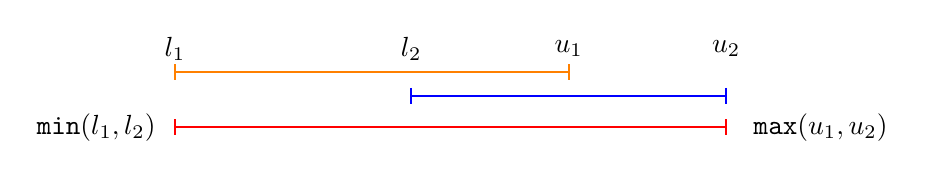
\begin{tikzpicture}
            %segmenti 
            \draw[thick, orange] (0, 0.5) -- (5, 0.5);
            \draw[thick, blue] (3, 0.2) -- (7, 0.2);
            \draw[thick, orange] (0, 0.6) -- (0, 0.4);
            \draw[thick, orange] (5, 0.6) -- (5, 0.4);
            \draw[thick, blue] (3, 0.3) -- (3, 0.1);
            \draw[thick, blue] (7, 0.3) -- (7, 0.1);
            %etichette
            \node at (0, 0.8) {$l_1$};
            \node at (5, 0.8) {$u_1$};
            \node at (3, 0.8) {$l_2$};
            \node at (7, 0.8) {$u_2$};
            %intervalli
            \draw[thick, red] (0, -0.2) -- (7, -0.2);
            \draw[thick, red] (0, -0.1) -- (0, -0.3);
            \draw[thick, red] (7, -0.1) -- (7, -0.3);
            %etichette
            \node at (-1, -0.2) {$\texttt{min}(l_1, l_2)$};
            \node at (8.2, -0.2) {$\texttt{max}(u_1, u_2)$};
        \end{tikzpicture}
    \end{figure}
    \item Greatest lower bound: ovvero il più grande intervallo contenuto
    in entrambi gli intervalli.
    \[
        [l_1, u_1] \sqcap [l_2, u_2] = [\texttt{max}(l_1, l_2), \texttt{min}(u_1, u_2)]
    \]
    \begin{figure}[H]
        \centering
        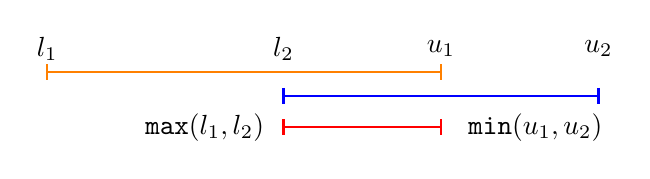
\begin{tikzpicture}
            %segmenti 
            \draw[thick, orange] (0, 0.5) -- (5, 0.5);
            \draw[thick, blue] (3, 0.2) -- (7, 0.2);
            \draw[thick, orange] (0, 0.6) -- (0, 0.4);
            \draw[thick, orange] (5, 0.6) -- (5, 0.4);
            \draw[thick, blue] (3, 0.3) -- (3, 0.1);
            \draw[thick, blue] (7, 0.3) -- (7, 0.1);
            %etichette
            \node at (0, 0.8) {$l_1$};
            \node at (5, 0.8) {$u_1$};
            \node at (3, 0.8) {$l_2$};
            \node at (7, 0.8) {$u_2$};
            %intervalli
            \draw[thick, red] (3, -0.2) -- (5, -0.2);
            \draw[thick, red] (3, -0.1) -- (3, -0.3);
            \draw[thick, red] (5, -0.1) -- (5, -0.3);
            %etichette
            \node at (2, -0.2) {$\texttt{max}(l_1, l_2)$};
            \node at (6.2, -0.2) {$\texttt{min}(u_1, u_2)$};
        \end{tikzpicture}
    \end{figure}
\end{itemize}
La descrizione di tali operazioni completa la descrizione del dominio, 
poiché siamo in presenza di un reticolo completo.

\subsection{Semantica delle espressioni}
Trattiamo ora del trasferimento del calcolo delle operazioni concrete nel 
dominio astratto, quindi definiamo la funzione di trasferimento astratta.
Tutte le operazioni possono essere trasferite, possiamo quindi fornire
in modo operativo sugli intervalli la \textbf{best correct approximation}
delle operazioni concrete. Definiamo alcune di queste operazioni:
\begin{itemize}
    \item $[l_1, u_1] +^\sharp [l_2, u_2] = [l_1 + l_2, u_1 + u_2]$ dove ricordiamo che 
    $-\infty + n = -\infty$ e $+\infty + n = +\infty$.
    \item $-^\sharp[l, u] = [-u, -l]$.
    \item $[l_1, u_1] \cdot^\sharp [l_2, u_2] = 
    [\texttt{min}(l_1 \cdot l_2, l_1 \cdot u_2, u_1 \cdot l_2, u_1 \cdot u_2), 
    \texttt{max}(l_1 \cdot l_2, l_1 \cdot u_2, u_1 \cdot l_2, u_1 \cdot u_2)]$.  
\end{itemize}
Nelle operazioni di confronto, per dire che due intervalli sono uguali,
dobbiamo essere sicuri che i loro valori nel dominio concreto lo 
siano, perciò due intervalli sono uguali se e solo se gli intervalli 
sono composti da un solo elemento e sono uguali, ovvero:
\[
  [l_1, u_1] =^\sharp [l_2, u_2] =
  \begin{cases}
    [1, 1] & \text{se } l_1 = u_1 = l_2 = u_2 \\
    [0, 0] & \text{se } u_i < l_2 \lor u_2 < l_1 \quad \textit{intervalli 
    disgiunti}\\
    [0, 1] & \text{altrimenti}
   \end{cases}
\]
Ciò significa che siamo assolutamente certi che due intervalli
sono uguali se e solo se sono composti da un solo elemento e sono uguali.
Sono sicuramente diversi se sono disgiunti, poiché nel corso dell'esecuzione 
hanno assunto valori totalmente diversi, rendendo impossibile per 
qualunque combinazione di valori che essi siano uguali. In tutti gli 
altri casi non possiamo essere certi che siano uguali, anche se i due 
intervalli sono uguali, poiché i valori nel dominio concreto potrebbero
essere diversi.

Definiamo quindi il dominio degli stati astratti negli intervalli come:
\[
  \mathbb{D} = (\texttt{Var} \to \mathbb{I}) \cup \{\bot\}
\]
Dove $\bot$ è indica uno stato non percorribile, oppure un errore.

Dato $\mathcal{D} \in \mathbb{D}$, definiamo la funzione di trasferimento
astratta $\alpha$ come la funzione che per ogni $x$ appartenente alle 
variabili, associa ad $x$, l'applicazione della funzione di trasferimento
astratta $\alpha$ all'intervallo associato ad $x$ in $\mathcal{D}$.
\[
   \alpha(\mathcal{D}) \implies \forall x \in \texttt{Var} 
   \quad x \mapsto \alpha(\mathcal{D})(x) 
\]
Estendendo quindi la funzione di trasferimento astratta $\alpha$ 
dalla funzione che opera sugli intervalli, alla funzione che opera
sugli stati che vogliono associare intervalli ai valori.

L'ordinamento rimane sempre quello definito per la propagazione 
delle costanti, quindi quando dobbiamo definire due stati astratti
si confronteranno i valori per ogni variabile.
Quindi:
\[
  \mathcal{D}_1 \sqsubseteq \mathcal{D}_2 \iff \forall x \in \texttt{Var} 
  \quad \mathcal{D}_1(x) \sqsubseteq_{intervalli} \mathcal{D}_2(x)
\]
L'obiettivo è avere questa informazione 
per ogni punto di programma, quindi cerchiamo la soluzione \texttt{MOP}, ovvero la
soluzione \textit{merge over all paths}, definendo quindi:
\[
    \texttt{MOP} : \mathcal{I}^\star [v] = \bigsqcup 
    \{ \llbracket \pi \rrbracket^\sharp \mathcal{D}_\bot \mid \pi:\text{start} \to v \}
\]
Ovvero il \textit{least upper bound}  (\textit{poiché la collecting semantics è di tipo possible}) 
delle semantiche di tutti i cammini a partire dall'informazione iniziale $\mathcal{D}_\bot$
dei cammini 
che vanno dal nodo di inizio al nodo $v$. È chiaro che se guardiamo tale analisi dal punto di vista delle 
analisi di data flow, l'analisi è forward, ed è di tipo possibile perché colleziona valori.

\subsection{Semantica dei comandi}
Descriviamo la semantica astratta dei comandi, sorvolando sulla semantica
delle espressioni, poiché è analoga alla definizione della semantica
astratta delle espressioni della propagazione delle costanti
(\ref{sec:semantica-espressioni}).

La semantica dei comandi ovviamente si baserà sulla semantica delle espressioni 
nel caso delle guardie e dell'assegnamento. Ragioniamo quindi induttivamente sulla
struttura dei comandi, definendo la semantica astratta dei comandi:
\begin{itemize}
    \item $\llbracket \texttt{;} \rrbracket^\sharp \mathcal{D} = \mathcal{D}$
    \item $\llbracket x \gets e \rrbracket^\sharp \mathcal{D} =
    \mathcal{D}[x \mapsto \llbracket e \rrbracket^\sharp \mathcal{D}]$
    \item $\llbracket \texttt{NonZero}(e) \rrbracket^\sharp \mathcal{D} =
    \begin{cases}
        \bot & \text{se } [0, 0] = \llbracket e \rrbracket^\sharp \\
        \mathcal{D} & \text{altrimenti}
    \end{cases}
    $
    \item $\llbracket \texttt{Zero}(e) \rrbracket^\sharp \mathcal{D} =
    \begin{cases}
        \bot & \text{se } [0, 0] \not \sqsubseteq \llbracket e \rrbracket^\sharp \\
        \mathcal{D} & \text{se } [0, 0] \sqsubseteq \llbracket e \rrbracket^\sharp
    \end{cases}
    $
    \item $\llbracket \texttt{input}(x) \rrbracket^\sharp \mathcal{D} =
    \mathcal{D}[x \mapsto \top ]$
\end{itemize}
Si può dimostrare che la semantica astratta $\llbracket \cdot \rrbracket^\sharp$ non 
è distributiva, quindi calcolando la soluzione \texttt{MFP} questa non sarà uguale 
alla soluzione \texttt{MOP}, ma la contiene strettamente.
\[
  \texttt{MFP} \sqsupseteq \texttt{MOP}  
\]
In ogni caso, la soluzione \texttt{MFP} è l'unica che riusciamo a costruire e l'analisi 
costruisce tale soluzione. 
Per farlo trova la soluzione del sistema di disequazioni, costruito esattamente come nel 
caso della analisi di data flow.
\begin{itemize}
    \item Sul nodo di partenza la memoria astratta è vuota, quindi
    \[
        \mathcal{I}[\texttt{entry}] \sqsupseteq \mathcal{D}_\bot 
    \]
    \item Per i nodi successivi, essendo una semantica forward, $\mathcal{D}[v]$ contiene 
    la semantica dell'etichetta a partire dalla memoria astratta a 
    partire dal nodo sorgente.
    \[
        \mathcal{I}[v] \sqsupseteq \llbracket \texttt{lab} \rrbracket^\sharp \mathcal{I}[u]
    \]
\end{itemize}
In ogni caso la semantica $\llbracket \cdot \rrbracket^\sharp$ è monotona, 
purtroppo non \texttt{ACC}, quindi contiene catene ascendenti infinite,
ma non abbiamo la garanzia di terminazione.
\begin{theorem}[Teorema di Knaster-Tarski]
    Sia $\mathcal{L}$ un reticolo completo, e sia $f : \mathcal{L} \to \mathcal{L}$ 
    una funzione monotona. Allora $f$ ha un punto fisso, ovvero un elemento $x \in \mathcal{L}$ 
    tale che $f(x) = x$.
\end{theorem}
La monotonia, per il teorema di Knaster-Tarski, ci garantisce che
esiste un punto fisso, ma non ci garantisce che sia raggiungibile
in un numero finito di passi.
\subsection{Migliorie all'analisi}
Possiamo pensare di migliorare l'analisi sapendo che la presenza di guardie la cui 
informazione calcolata è rappresentabile all'interno della nostra osservazione.
\begin{itemize}
    \item 
    \[
      \llbracket \texttt{NonZero}(e) \rrbracket^\sharp \mathcal{D} =
    \begin{cases}
        \bot & \text{se } [0, 0] = \llbracket e \rrbracket^\sharp \\
        \mathcal{D}_1 & \text{altrimenti}
    \end{cases}  
    \]
    Dove $\mathcal{D}_1$ è può essere:
    \[
        \mathcal{D}_1 = \begin{cases}
            \mathcal{D}[x \mapsto \mathcal{D}(x) \sqcap \llbracket e_1 \rrbracket^\sharp] & 
            \text{se } e \equiv (x = e_1) \\
            \mathcal{D}[x \mapsto \mathcal{D}(x) \sqcap [-\infty, -u - 1]] &
            \text{se } e \equiv (e_1 < x) \text{ e } \llbracket e_1 \rrbracket^\sharp = [l, u] \\
            \mathcal{D}[x \mapsto \mathcal{D}(x) \sqcap [l + 1, +\infty]] &
            \text{se } e \equiv (x > e_1) \text{ e } \llbracket e_1 \rrbracket^\sharp = [l, u] \\
        \end{cases}
    \] 
    \item Il caso di \texttt{Zero} è analogo.
\end{itemize}
Ovviamente, la condizione vale se $e$ è del tipo $x \,\square \,e_1$, 
dove il simbolo $\square$ può essere $\{ =, <, > \}$.
\subsubsection{Esempio di analisi degli intervalli}

Consideriamo il seguente programma:

\begin{algorithm}[H]
    \If{$x \geq 0$}{
        $y \gets 0$ \;
    }
    \Else{
        \While{$x < 0$}
        {
            $x \gets x + 1$ \;
            $y \gets x$ \;
        }
    }
\end{algorithm}

    \begin{figure}[H]
        \centering
        \begin{tikzpicture}[node distance={22mm}, minimum width = 1cm, main/.style = {draw, circle}] 
            \node[main] (1) {1};
            \node[main] (2) [below left=of 1] {2};
            \node[main] (3) [below =of 2] {3};
            \node[main] (4) [below right=of 1] {4};
            \node[main] (5) [below right=of 4] {5};
            \node[main] (6) [below =of 5] {6};
            \node[main] (7) [below left=of 4] {7};
            \node[main] (8) [below =of 7] {8};
            
            \draw[->] (1) -- (2) node[midway, left] {\small$\texttt{NonZero}(x \geq 0)$};
            \draw[->] (2) -- (3) node[midway, left] {\small$y \gets 0$};
            \draw[->] (1) -- (4) node[midway, right] {\small$\texttt{Zero}(x \geq 0)$};
            \draw[->] (4) -- (5) node[midway, right] {\small$x < 0$};
            \draw[->] (5) -- (6) node[midway, right] {\small$x \gets x + 1$};
            \draw[->] (6) -- (4);
            \draw[->] (4) -- (7) node[midway, left] {\small$\texttt{Zero}(x < 0)$};
            \draw[->] (7) -- (8) node[midway, right] {\small$y \gets x$};
            \draw[->] (3) -- (8) node[midway, left] {\small$;$};
        \end{tikzpicture}
    \end{figure}

Dobbiamo costruire il sistema di disequazioni, che possiamo
riportare già in forma di equazioni:
\begin{itemize}
    \item $\mathcal{I}(1) = \mathcal{I}_\bot$
    \item $\mathcal{I}(2) = \mathcal{I}(1) \sqcap \mathcal{I}_\bot [x \mapsto [0, +\infty]] =
    \mathcal{I}(1) \sqcap [x \mapsto [0, +\infty]]$
    \item $\mathcal{I}(3) = \mathcal{I}(2) [y \mapsto [0, 0]]$
    \item $\mathcal{I}(4) = \mathcal{I}(1) \sqcap [x \mapsto [-\infty, -1]] \sqcup 
    \mathcal{I}(6)$
    \item $\mathcal{I}(5) = \mathcal{I}(4) \sqcap [x \mapsto [-\infty, -1]]$
    \item $\mathcal{I}(6) = \mathcal{I}(5) [x \mapsto \mathcal{I}(5)(x) +^\sharp [1, 1]]$
    \item $\mathcal{I}(7) = \mathcal{I}(4) \sqcap [x \mapsto [0, +\infty]]$
    \item $\mathcal{I}(8) = \mathcal{I}(7) [y \mapsto \mathcal{I}(7)(x)]
    \sqcup \mathcal{I}(3)$
\end{itemize}
Possiamo quindi calcolare il punto fisso:
\begin{table}[H]
    \centering
    \begin{subtable}{\linewidth}
        \centering
        \begin{tabular}{|c|c|c|c|}
            \hline
            & $0$ 
            & $1$ 
            & $2$ \\ \hline
            $\mathcal{I}(1)$ 
            & $\mathcal{I}_\bot$ 
            & $\mathcal{I}_\bot$ 
            & $\mathcal{I}_\bot$ \\
            \hline
            $\mathcal{I}(2)$ 
            & $\varnothing$ 
            & $[x \gets [0, +\infty], y \gets \top]$ 
            & $[x \gets [0, +\infty], y \gets \top]$ \\
            \hline
            $\mathcal{I}(3)$ 
            & $\varnothing$ 
            & $[x \gets [0, +\infty], y \gets [0, 0]]$
            & $[x \gets [0, +\infty], y \gets [0, 0]]$ \\
            \hline
            $\mathcal{I}(4)$ 
            & $\varnothing$ 
            & $[x \gets [-\infty, -1], y \gets \top]$
            & $[x \gets [-\infty, 0], y \gets \top]$ \\
            \hline
            $\mathcal{I}(5)$ 
            & $\varnothing$ 
            & $[x \gets [-\infty, -1], y \gets \top]$
            & $[x \gets [-\infty, -1], y \gets \top]$ \\
            \hline
            $\mathcal{I}(6)$ 
            & $\varnothing$ 
            & $[x \gets [-\infty, 0], y \gets \top]$
            & $[x \gets [-\infty, 0], y \gets \top]$ \\
            \hline
            $\mathcal{I}(7)$ 
            & $\varnothing$ 
            & $\bot$
            & $[x \gets [0, 0], y \gets \top]$ \\
            \hline
            $\mathcal{I}(8)$ 
            & $\varnothing$ 
            & $\bot$
            & $[x \gets [0, +\infty], y \gets [0, 0]]$ \\
            \hline
        \end{tabular}
    \end{subtable}
\end{table}
Dove raggiungiamo il punto fisso in $2$ iterazioni.
\section{Widening}
Il \textit{widening} è un'operazione che accelera le computazioni a punto fisso garantendo
la convergenza. L'operatore di widening consente di eseguire ``salti" per raggiungere
un punto fisso approssimato.

Dato un dominio $\mathbb{P}$ su cui è definito un poset, il widening è una funzione:

\[
\nabla : \mathbb{P} \times \mathbb{P} \rightarrow \mathcal{P}
\]

dove:

\[
\forall x,y \in \mathbb{P} . \quad x \sqsubseteq (x \nabla y) \land y \sqsubseteq (x \nabla y)
\]

L'applicazione dell'operatore deve mantenere un certo ordine. Inoltre, quando definiamo
ad hoc l'operatore di widening, le catene ascendenti devono essere convergenti.

Supponiamo di avere una catena del tipo:

\[
x_0 \sqsubseteq x_1 \sqsubseteq x_2 \sqsubseteq \dots \sqsubseteq x_n \sqsubseteq \dots
\]

La costruzione di una nuova catena, chiamata $y$, è definita come:

\[
y_0 = x_0 \quad y_1 = x_1 \nabla y_0 \quad y_{2} = x_2 \nabla y_1 \quad \dots \quad y_n
= x_n \nabla y_{n-1} \quad \dots
\]

L'elemento precedente della nuova catena deve essere combinato con il nuovo elemento della
catena precedente, dove $y_i$ è una catena non strettamente crescente ma che converge a
un punto fisso.

La definizione del concetto di widening potrebbe risultare poco esplicativa in questo
contesto; tuttavia, se si considerano le disequazioni nella forma

\[
  x_i \sqsubseteq f_i(x_1, \dots, x_n)
\]

e si applica la definizione di contenimento,

\[
  x_i \sqsubseteq f_i(x_1, \dots, x_n) \iff x_i = x_i \sqcup f_i(x_1, \dots, x_n)  
\]

sostituendo l'operatore di widening all'operatore di least upper bound, si ottiene

\begin{equation}
    x_i = x_i \nabla f_i(x_1, \dots, x_n)
\end{equation}

Questo sistema di disequazioni assicura la costruzione di una catena convergente al punto fisso,
garantendo nel contempo la terminazione (\textit{sotto l'assunzione delle proprietà specificate}).

L'idea di fondo è quella di fornire un operatore che sostituiamo al least upper bound. 
Il least upper bound, per costruzione, essendo la più piccola soluzione, fa si che si 
possa divergere poiché prende in considerazione tutti gli elementi della catena.
Il widening, invece, è un operatore che si comporta come un least upper bound ma che
non prende in considerazione tutti gli elementi della catena, ma una sottocatena 
che converge al punto fisso.
Perciò l'operazione di widening è un'operazione che viene utilizzata in combinazione 
con l'operazione di \texttt{narrowing} per garantire la terminazione. Che a partire 
dalla soluzione del widening, ovvero una soluzione estremamente approssimata, 
cerca di capire se il calcolo aveva informazioni che in realtà possono essere
sfruttate per affinare la soluzione. 
\subsection{Widening per gli intervalli}
